\documentclass[11pt]{article}
\usepackage{geometry}                % See geometry.pdf to learn the layout options. There are lots.
\geometry{letterpaper}                   % ... or a4paper or a5paper or ... 
%\geometry{landscape}                % Activate for for rotated page geometry
%\usepackage[parfill]{parskip}    % Activate to begin paragraphs with an empty line rather than an indent
\usepackage{graphicx}
\usepackage{color}
\usepackage{amssymb}
\usepackage{epstopdf}
\usepackage{amsmath}
\usepackage{sectsty}
\usepackage{algorithm}
\usepackage{algorithmic}
\usepackage[hyphens]{url}  %% be sure to specify the option 'hyphens'
\DeclareGraphicsRule{.tif}{png}{.png}{`convert #1 `dirname #1`/`basename #1 .tif`.png}

\title{Drake-Cullen-Assignment5}
\author{Drake Cullen}
%\date{}                                           % Activate to display a given date or no date

\newcommand\tab[1][1cm]{\hspace*{#1}}

\begin{document}
%\maketitle
%\section{}
%\subsection{}
\begin{minipage}{\linewidth}% to keep image and caption on one page
\centering

\includegraphics[keepaspectratio=true,scale=0.35]{CMU.png}
\end{minipage}
\section*{ \centering Assignment 5}
\subsection*{ \centering By Drake Cullen} 

\vspace{5mm}
 
I declare that all material in this assessment task is my work except where there is clear acknowledgement or reference to the work of others. I further declare that I have complied and agreed to the CMU Academic Integrity Policy at the University website. http://www.coloradomesa.edu/student-services/documents
\begin{center}
\textbf{Author’s Name:} Drake Cullen 
\textbf{UID(700\#):} 700480375
\textbf{ Date:} 11/23/2021
\end{center} 

\section{Chapter 3, Question 1)}
Topological sorting is an ordering of vertices in the manner that  for every directed edge u v, the vertex u comes before v in the ordering (Kleinberg, 2014, p. 99). In figure 3.10, there are a total of 6 unique topological orderings. We know that f will always be the last node, a is always the first node, c relies on b, and e relies on d. Here are the 6 topological orderings:

\begin{align*}
a, b, c, d, e, f \\
a, b, d, c, e, f\\
a, b, d, e, c, f\\
a, d, e, b, c, f\\
a, d, b, e, c, f\\
a, d, b, c, e, f \\
\end{align*}

\section{Chapter 3, Question 2)}
In class, we learned that a graph contains a cycle if the graph contains a backward edge. The DFS algorithm can be run on the graph to perform edge classification. A backward edge will appear if there is a connection from a node to its ancestor (Antoun, "More on DFS").


\begin{algorithm}[H]
\caption{DFS\_Cycle(graph, vertex, visited, parent)}
\begin{algorithmic} 
\STATE // return true if a cycle (backward edge) is found
\STATE visited[vertex] = true
\FOR{neighbor in adj[vertex]}
\IF{neighbor not in visited}
\IF{DFS\_Cycle(graph, neighbor, visited, vertex}
\RETURN true
\ENDIF
\ELSE
\IF{neighbor not equal to parent}
\RETURN true
\ENDIF
\ENDIF
\ENDFOR
\RETURN false
\end{algorithmic}
\end{algorithm}

If the algorithm above returns true, we need to print out the cycle. To do this, start at the node with a backward edge. Continually return to the previous node until the paths end up at the same node. You can then print these nodes in the correct order to showcase the cycle.

\section{Chapter 3, Question 3)}
According to the proof on page 102, "In every DAG G, there is a node v with no incoming edges" (Kleinberg, 2014). In the solution provided by the book, we continually remove nodes with no incoming nodes. To address the general case where the graph may not be a DAG, we check to see if there is at least one node with no incoming edges in every iteration of the algorithm. If there is not a node with no incoming edges, we know that the graph isn't a DAG and we will print out the cycle. The cycle will be printed by continually visiting the node that led to this node until we come across a repeat node. This list of nodes forms a cycle. \newline In the other case where there is a least one node in every iteration with no incoming edges, the algorithm needs no modifications and will print out the topological ordering.

\section{Chapter 4, Question 1)}
The statement is \textbf{True}. In the lecture, "Graphs - Introduction," we analyzed two techniques to form a Minimum Spanning Tree. One of the methods followed the strategy of adding an edge at a time and is known as Kruskal's algorithm. At each stage, the edge with the smallest weight is added as long as it doesn't create a cycle  (Antoun, 2021). If e* is the edge with the smallest weight then it must be part of an MST because it would be the first edge to be added in Kruskal's algorithm.

\section{Chapter 4, Question 2)}
\subsection{}
The statement is \textbf{True} because it follows a similar argument that the last question did. If the cost of each edge in the graph is squared, the edges stay in the same relative order to one another. For instance, $ 2 < 3 $ and $ 2^{2} < 3^{2} $. Now if Kruskal's algorithm is ran on the squared edges, it will produce the same MST that the original input would produce.
\subsection{}
The statement is \textbf{False}. For example, weights with a value of one can cause a problem because the weights won't increase proportionally. The statement would be true if every weight was multiplied by a constant such as 2. The manner in which the statement fails can be seen in the example below. 

\begin{center}
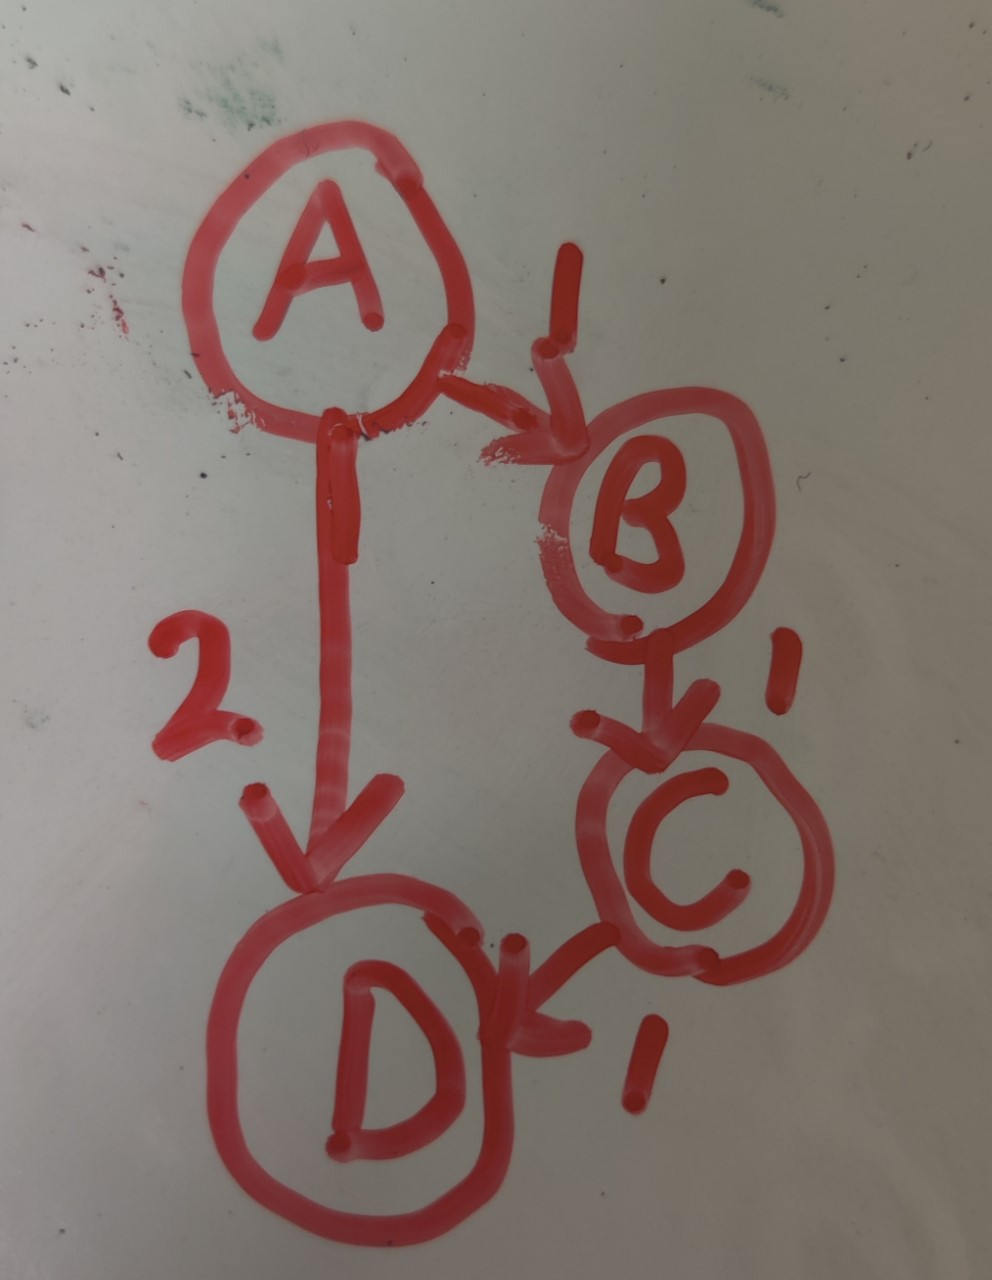
\includegraphics[keepaspectratio=true,scale=0.25]{graph2.jpg}
\end{center}
Let us assume that you are looking for the shortest path from A to D using the graph above. There are two different paths that you can take to get from A to D.

\begin{center}
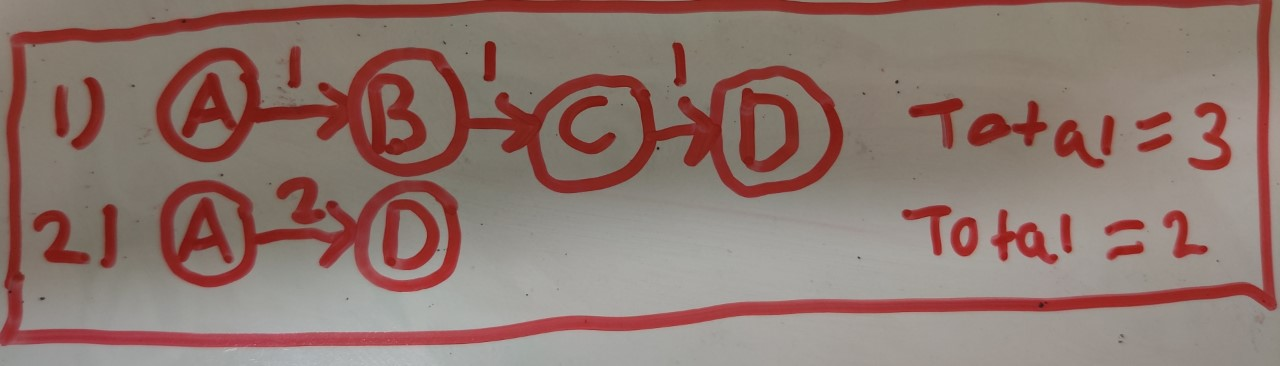
\includegraphics[keepaspectratio=true,scale=0.25]{original_paths2.jpg}
\end{center}
By taking the path from A to B to C to D (call this path1), the combined weight is 3. If you choose to take the path2 from A to D, the combined weight is 2. Therefore, path2 is shorter than path1.

\begin{center}
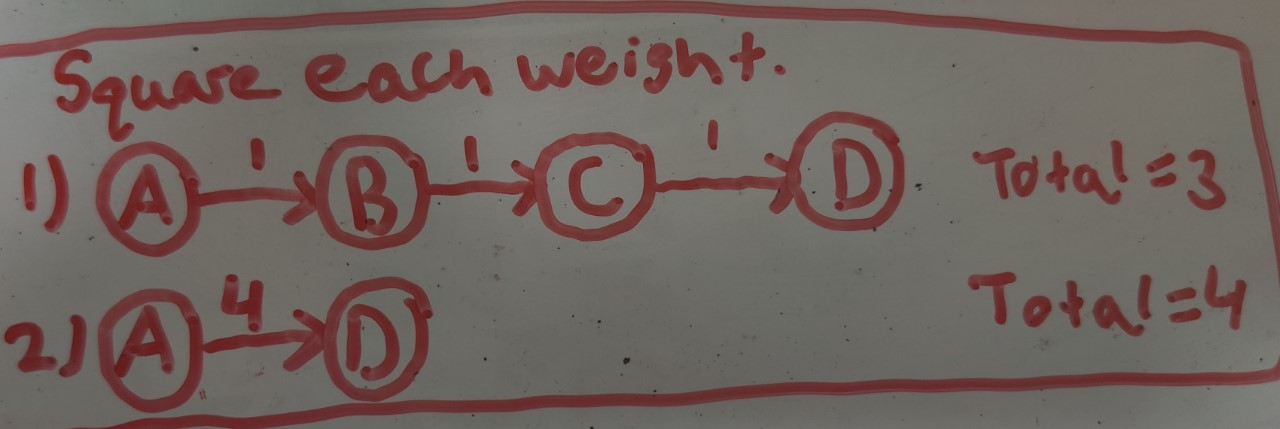
\includegraphics[keepaspectratio=true,scale=0.25]{updated_paths2.jpg}
\end{center}
After squaring every edge, the updated paths can be seen in the image above. Path1 is now shorter than path2. We know that path2 should be shorter than path1, so by squaring every edge, the shortest path is now innacurate; therefore, this statement is false.

\section{Chapter 4, Question 4)}
\begin{algorithm}[H]
\caption{Detect\_Subsequence(s, sPrime)}
\begin{algorithmic} 
\STATE // return true if S' is a subsequence of S
\STATE sIndex = sPrimeIndex = 0
\WHILE{sIndex $<$ length(s) and sPrimeIndex $<$ length(sPrime)}
\IF{s[sIndex] == sPrime[sPrimeIndex]}
\STATE sIndex++
\STATE sPrimeIndex++
\ELSE
\STATE sIndex++
\ENDIF
\ENDWHILE
\IF{sPrimeIndex == length(sPrime)}
\RETURN true
\ENDIF
\RETURN false
\end{algorithmic}
\end{algorithm}

The algorithm works by having two indices. One of the indices points to the current word in S and the other points to the current word in S'. Every time that the word in S matches the word in S', each index increases by one. The S pointer increments by one every time through the loop. In summary, the algorithm tries to find the current word of S' in S. Upon finding the word in S, the algorithm moves on to the next word in S'. If we reach the end of S', we know that all of the words were found; thus, the algorithm returns true.
\newline
In every iteration of the loop, at least one of the indexes increments. In the worst case, the loop will go through every word in S. If we iterate over every word where S has length n and S' has length m, the runtime will be O(n) which is linear.

\section{Chapter 5, Question 3)}
In this problem, we are trying to determine if at least half of the cards have the same value. If they do, then there is a majority element. To solve this problem, we can repeatedly break the number of elements into two groups. If at least half of the cards in a group have the same element, then it will return a card with that value. We know that if there is a majority card, at least one of the halves will have a majority of that card. 
\newline 
If we hit the base case of one card, that card is returned. If the two halves have the same majority card, that card is returned. Otherwise, the subsets must be searched to see which card appears more. Whichever card appears more is returned.
\begin{algorithm}[H]
\caption{Is\_Majority\_Element(cards, low, high)}
\begin{algorithmic} 
\IF{low == high}
\RETURN cards[low]
\ENDIF
\STATE middle = (high - low) / 2 + low
\STATE leftMajority = Is\_Majority\_Element(cards, low, middle)
\STATE rightMajority = Is\_Majority\_Element(cards, middle + 1, high)
\IF {leftMajority == rightMajority}
\RETURN leftMajority
\ENDIF
\STATE leftCount = the number of times leftMajority appears
\STATE rightCount = the number of time RightMajority appears
\IF{leftCount $>$ rightCount}
\RETURN leftMajority
\ELSE
\RETURN RightMajority
\ENDIF
\end{algorithmic}
\end{algorithm}

From working with previous problems, we know that repeatedly dividing a set into two will take log(n) runtime. In each division, we may have to compare with up to n elements; therefore, the runtime complexity is O(n*log(n))

\section{Chapter 6, Question 1)}
\subsection{}
The "heaviest-first" greedy algorithm does not always find an independent set of maximum total weight. For instance, say that we have a graph G with 3 nodes. In this graph, V$_1$ = 7, V$_2$ = 8, and V$_3$ = 7. The heaviest-first algorithm will pick V$_2$ and the weight of the independent set will be 8. This answer is incorrect because V$_1$ and V$_2$ could be picked to give a weight of 14.

\subsection{}
The algorithm that looks at the maximum weight between S$_1$ and S$_2$ where S$_1$ is the set of all odd number nodes and S$_2$ is the set of all even number nodes does not always find an independent set of maximum total weight. For example, consider figure 6.28. The nodes in order have weights 1, 8, 6, 3, 6. S$_1$ will consist of 1, 6, 6 for a total of 13 and S$_2$ will have the elements 8, 3 for a total of 11. The actual maximum independent set would choose items 8 and 6 for a total weight of 14.

\subsection{}
As we iterate over every node, there are two options: the node is included or it isn't included. If the node is included, we have to remove the last node. Our current weight will be equal to the weight of two nodes back, plus the weight added for including this node. Otherwise, if the node isn't included, the weight will be the same as the last iteration (when we didn't have this node). This process is seen in the following algorithm.

\begin{algorithm}[H]
\caption{Calculate\_Max\_Weight(nodeWeights)}
\begin{algorithmic} 
\STATE maxWeights is an empty array with the length the same as nodeWeights length
\STATE maxWeights[0] = 0
\STATE maxWeights[1] = nodeWeights[0]
\FOR{i in range len(nodeWeights)}
\STATE maxWeights[i] = maximum(maxWeights[i-1], maxWeights[i - 2] + nodeWeights[i]
\ENDFOR
\RETURN nodeWeights[len(nodeWeights)]
\end{algorithmic}
\end{algorithm}


\section{Chapter 7, Question 2)}
\subsection{}
The value of the flow is 18. No, this is not a maximum flow. The maximum flow is 21.
\subsection{}
The minimut s-t cut eliminates the edges shown in red in the following image. Two independent sets are formed, and s and t are in seperate sets. The capacity is 21.
\begin{center}
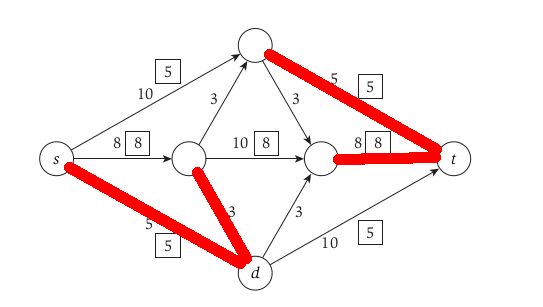
\includegraphics[keepaspectratio=true,scale=0.5]{9Cut.png}
\end{center}

\section{Chapter 7, Question 3)}
\subsection{}
The value of the flow is 10. No, this is not a maximum flow. The maximum flow is 11.
\subsection{}
The minimut s-t cut eliminates the edges shown in red in the following image. Two independent sets are formed, and s and t are in seperate sets. The capacity is 11.
\begin{center}
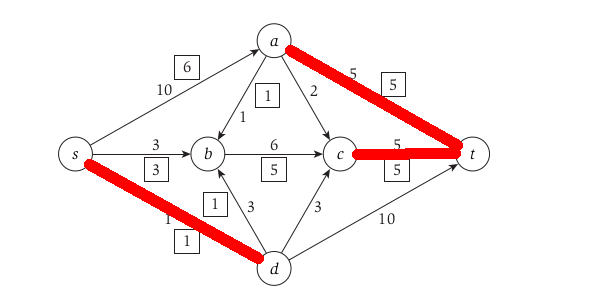
\includegraphics[keepaspectratio=true,scale=0.5]{10Cut.png}
\end{center}

\begin{thebibliography}{1}

\bibitem{impj} Kleinberg, Jon and Tardos Eva. Algorithm Design. Pearson, 2014. 
\bibitem{impj} Antoun, Sherine (2021, September 15). More on DFS [Lecture].
\bibitem{impj} Antoun, Sherine (2021, September 8). Graphs - Introduction [PowerPoint].

 \end{thebibliography}


\end{document}  